% !TEX root = thesis.tex

%%
%%
%% Discussion chapter
%%
%%

The contribution of this thesis is an empirical statistical analysis of the accuracy of the \gls{dkd}
as a tool for estimating the incidence risk of chronic diseases.
We examined the effect of several factors on the \gls{dkd} accuracy,
and we measured the accuracy of the \gls{dkd} using \gls{mise},
\gls{miae}, \gls{supremum error}, as well as \gls{peak bias}, \gls{peak drift} and \gls{centroid bias} and \gls{centroid drift},
as described in \Cref{sec:method:accuracy}.
We ran several scenarios to examine how variations in these factors which affect the incidence risk function,
the population distribution, and the sample size affect the accuracy of \gls{dkd} for estimation.
We compared two bandwidth selection techniques, \gls{silverman}'s rule of thumb,
and least-squares \glsentrylong{cv}.
We also compared these two techniques to an \gls{oracle},
which is an approximation of the theoretical optimal bandwidth,
keeping in mind that the oracle is only computable for simulations because we know the true function we wish to estimate.

In order to discuss the overall accuracy of all of the experiments,
we divided the experiments into two groups.
The first group, which comprises most of the experiments,
consist of different \gls{risk} functions on \textbf{uniform populations}.
The second group consists of different \gls{risk} functions on population distributions with a \textbf{single peak}.
The results of the second group are found in \Cref{sec:results:pop_spread} while the results of the first group comprise the remainder.
In general, the estimation errors observed for the first group of experiments were much higher than the second.
This indicates that the population distribution has a noticeable negative effect on the accuracy of the \gls{dkd}.

As we discussed in \Cref{subsec:method:mise},
the \glsentrylong{mise} is the measure used by both \gls{silverman} and \gls{cv} for choosing the bandwidth.
In order to compare the results of different experiments which differ in the scales of their \gls{risk} functions,
we compute the normalized \gls{mise}, or \gls{nmise}. 
\Cref{fig:discussion:overall_nmise_boxplot} shows the overall distribution between experiments of the \gls{nmise}.
The \gls{nmise} for the \gls{oracle} selected bandwidth was, on average,
lower than for the other bandwidth selectors.
The \gls{cv} and \gls{silverman} selectors had similar performance.
All of these bandwidth selection techniques are optimized to minimize \gls{mise},
and so these results are what we expected.

The scale of the \gls{nmise} is much higher for the non-uniform population group of experiments.
In particular, this seems to happen in two scenarios.
The first scenario occurs when the \gls{risk} function peak is far from the population peak, resulting in very few people in the high-risk area,
as in \Cref{sec:app:results_p1.4_100_1_1h_X}.
In a study with a real \gls{incident} \gls{risk},
this would have the effect of producing a very low number of observed \glspl{incident}.
The resulting estimated \gls{risk} would then have high variance even when normalized.
The second scenario where the \gls{nmise} is high occurs when the population density \gls{spread} takes its lowest values of 0.7 and 1.0.
This results in a highly variable denominator in the \gls{dkd} quotient,
leading to less stable results.

\begin{figure}[htbp]
    \centering
    \begin{subfigure}[t]{0.45\textwidth}
        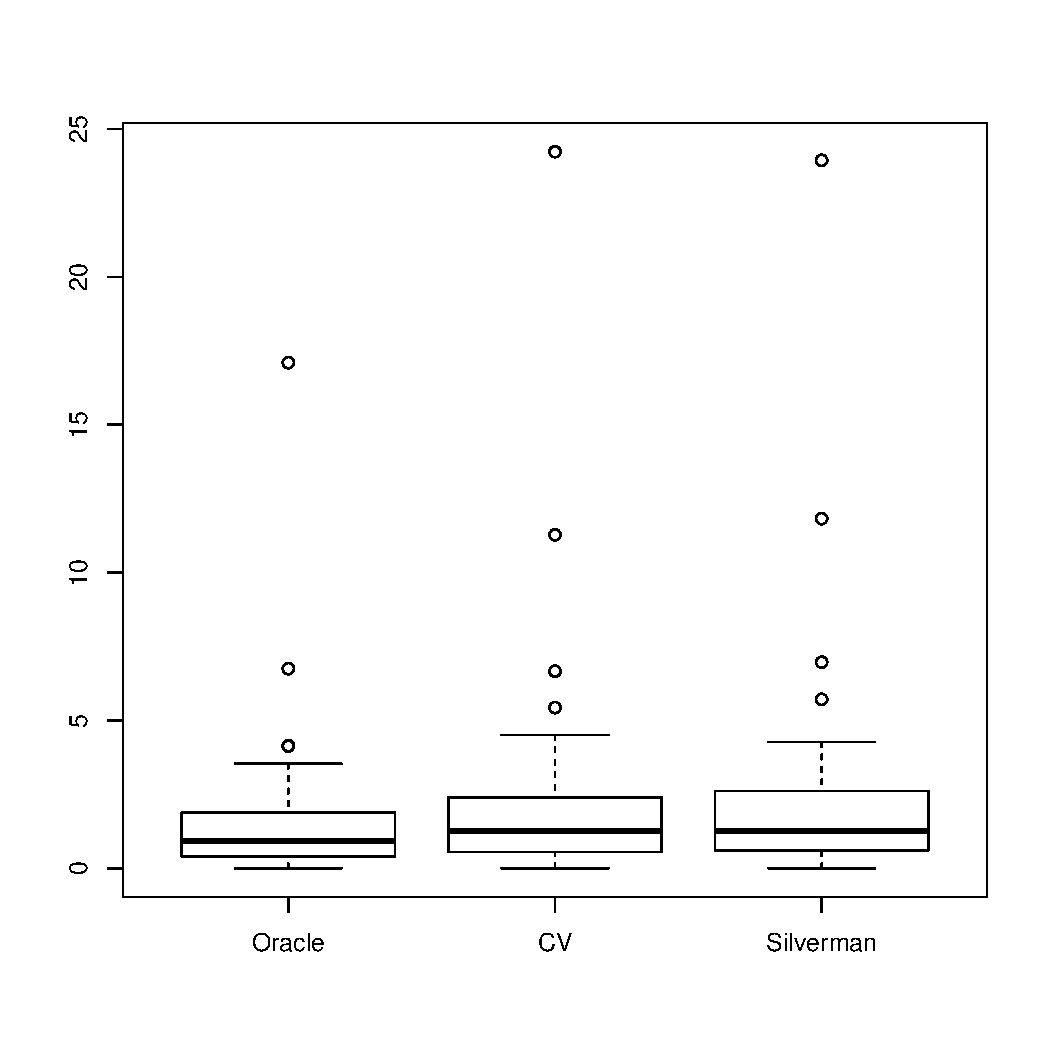
\includegraphics[width=\textwidth]{results/by_overall/normalized-mise-boxplot}
        \subcaption{Uniform populations}
        \label{fig:discussion:overall_nmise_boxplot:unif}
    \end{subfigure}
    \begin{subfigure}[t]{0.45\textwidth}
        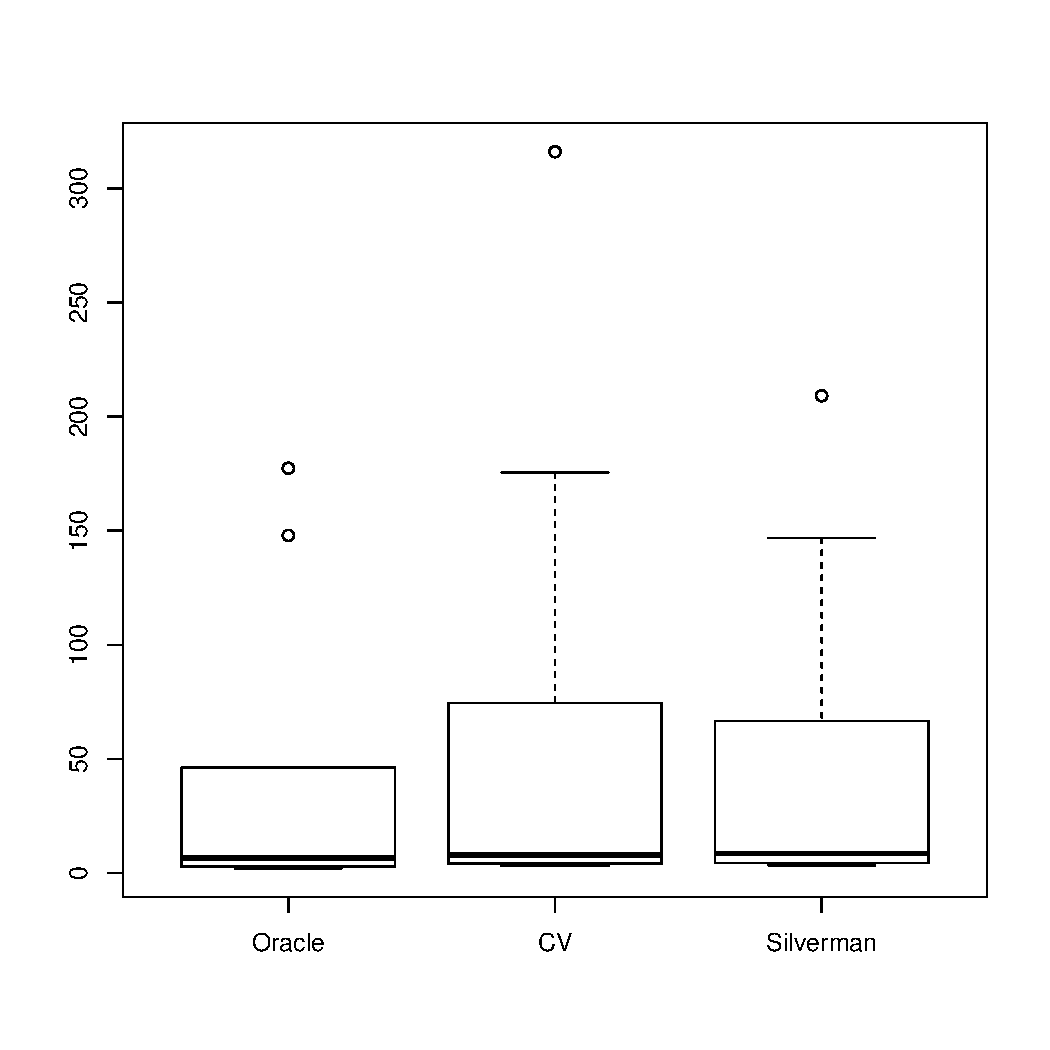
\includegraphics[width=\textwidth]{results/by_overall/normalized-mise-peakpop-boxplot}
        \subcaption{Peaked populations}
        \label{fig:discussion:overall_nmise_boxplot:peak}
    \end{subfigure}
    \caption[Overall distribution of \glsentryname{nmise}]
        {Overall distribution of \glsentryname{nmise}.
            The error scale in \autoref{fig:discussion:overall_nmise_boxplot:peak} is higher by a factor of 15.}
    \label{fig:discussion:overall_nmise_boxplot}
\end{figure}

\begin{figure}[htbp]
    \centering
    \begin{subfigure}[t]{0.45\textwidth}
        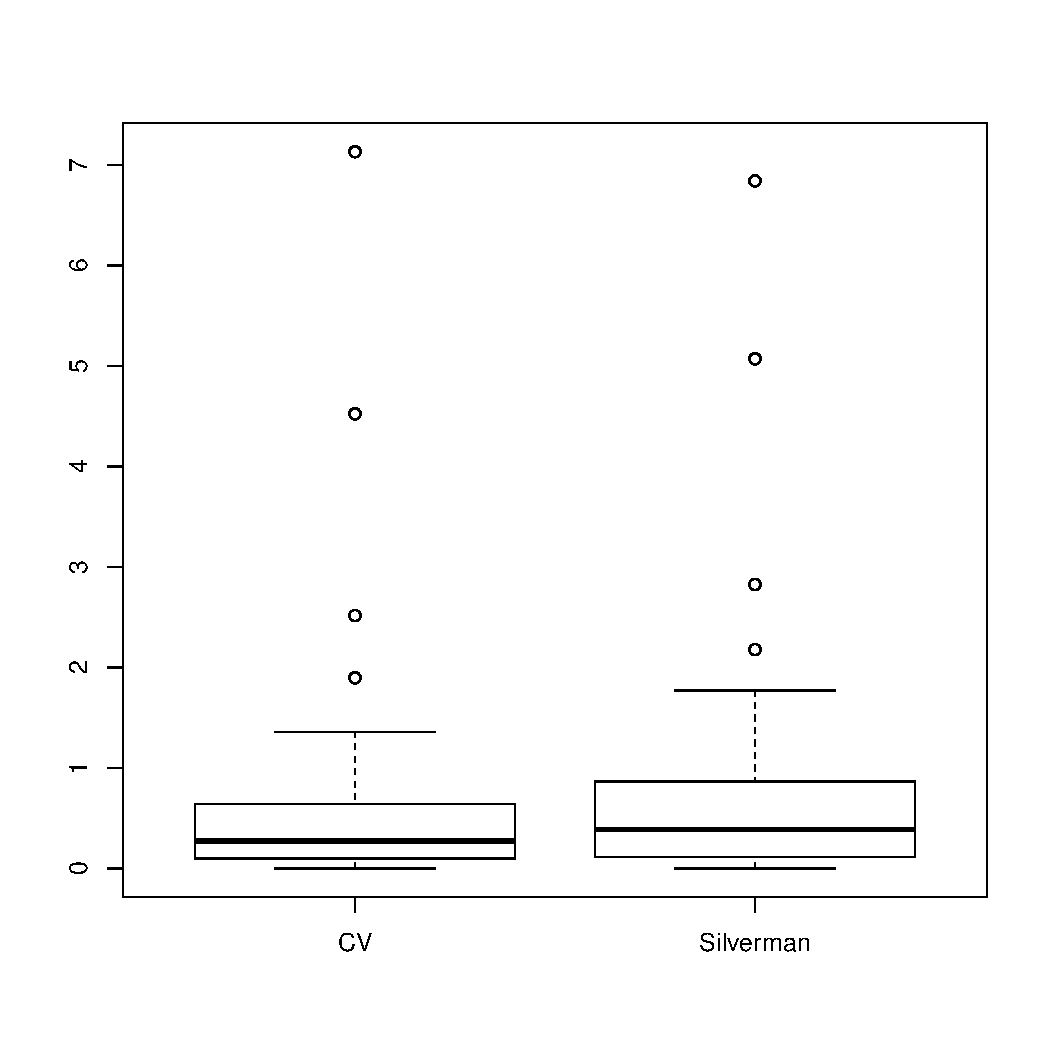
\includegraphics[width=\textwidth]{results/by_overall/normalized-mise-diff-boxplot}
        \subcaption{Uniform populations}
        \label{fig:discussion:overall_nmise_diff_boxplot:unif}
    \end{subfigure}
    \begin{subfigure}[t]{0.45\textwidth}
        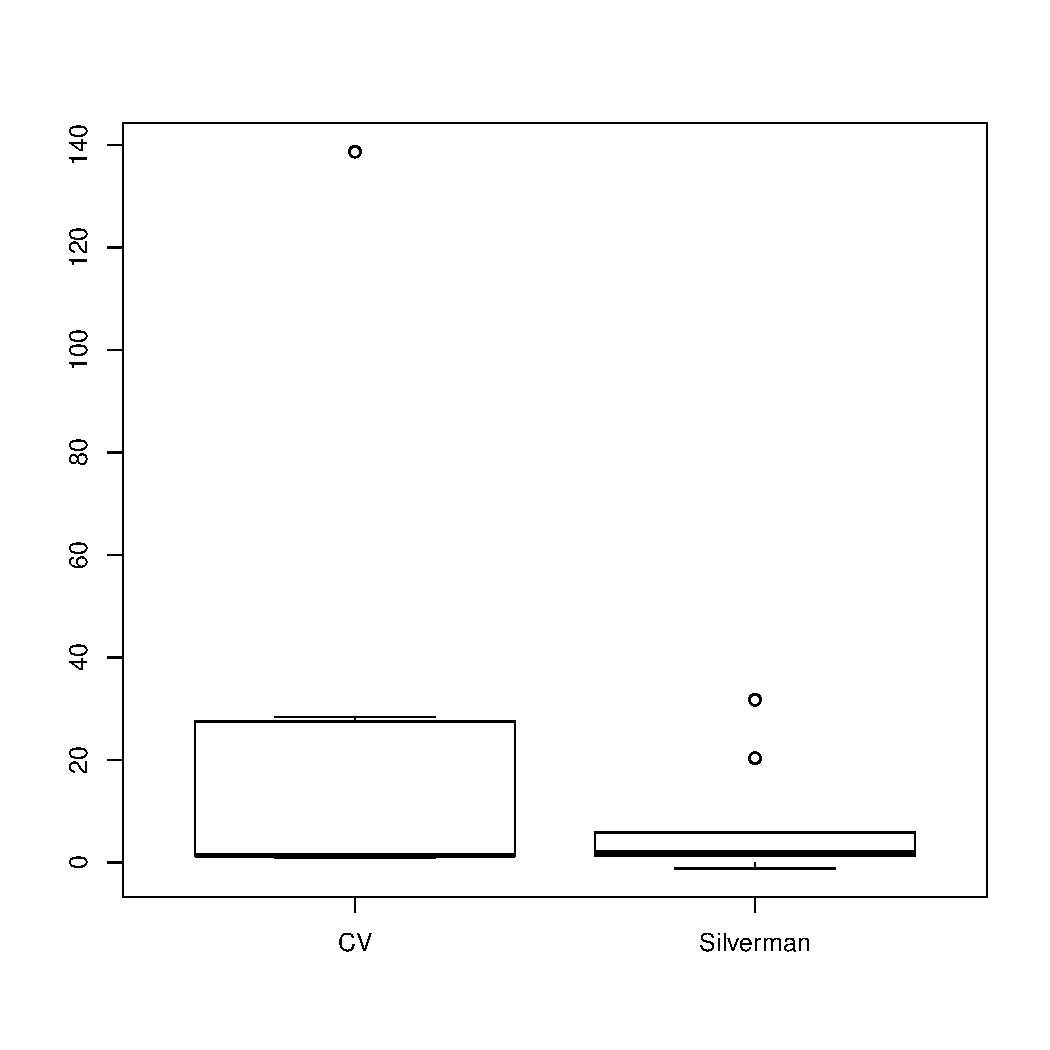
\includegraphics[width=\textwidth]{results/by_overall/normalized-mise-diff-peakpop-boxplot}
        \subcaption{Peaked populations}
        \label{fig:discussion:overall_nmise_diff_boxplot:peak}
    \end{subfigure}
    \caption[Overall distribution of \glsentryname{nmise} difference from the \Glsentryname{oracle}]
        {Overall distribution of \glsentryname{nmise} difference from the \Glsentryname{oracle}.
            The error scale in \autoref{fig:discussion:overall_nmise_boxplot:peak} is higher by a factor of 20.}
    \label{fig:discussion:overall_nmise_diff_boxplot}
\end{figure}

We now look at the \gls{miae}.
As mentioned in \Cref{subsec:method:miae},
the \glsentrylong{miae} is the natural measure that shows the average overall accuracy of the \gls{dkd} estimate of the \gls{risk} function.
By normalizing the \gls{miae}, we obtain the \gls{nmiae}.
Our theoretical optimal bandwidth \gls{h_opt} and our \gls{oracle} which is our estimation of it,
are based on minimizing \gls{mise}.
Also, both of \gls{silverman} and \gls{cv} are bandwidth selectors that attempt to minimize \gls{mise}.
It is not necessarily the case that a bandwidth that minimizes \gls{ise} may also be the minimizer of \gls{iae}.
Nevertheless, our results show that for the types of \gls{risk} intensities we studied,
the \gls{cv} and \gls{silverman} selectors performed similarly to each other for \gls{nmiae}.
\Cref{fig:discussion:overall_nmiae_boxplot} shows the distribution of \gls{nmiae} over the entire set of experiments.
We note the large difference in scale between the experiments with uniform populations shown in \subref{fig:discussion:overall_nmiae_boxplot:unif} and those with peaked populations in \subref{fig:discussion:overall_nmiae_boxplot:peak}.


\begin{figure}[htbp]
    \centering
    \begin{subfigure}[t]{0.45\textwidth}
        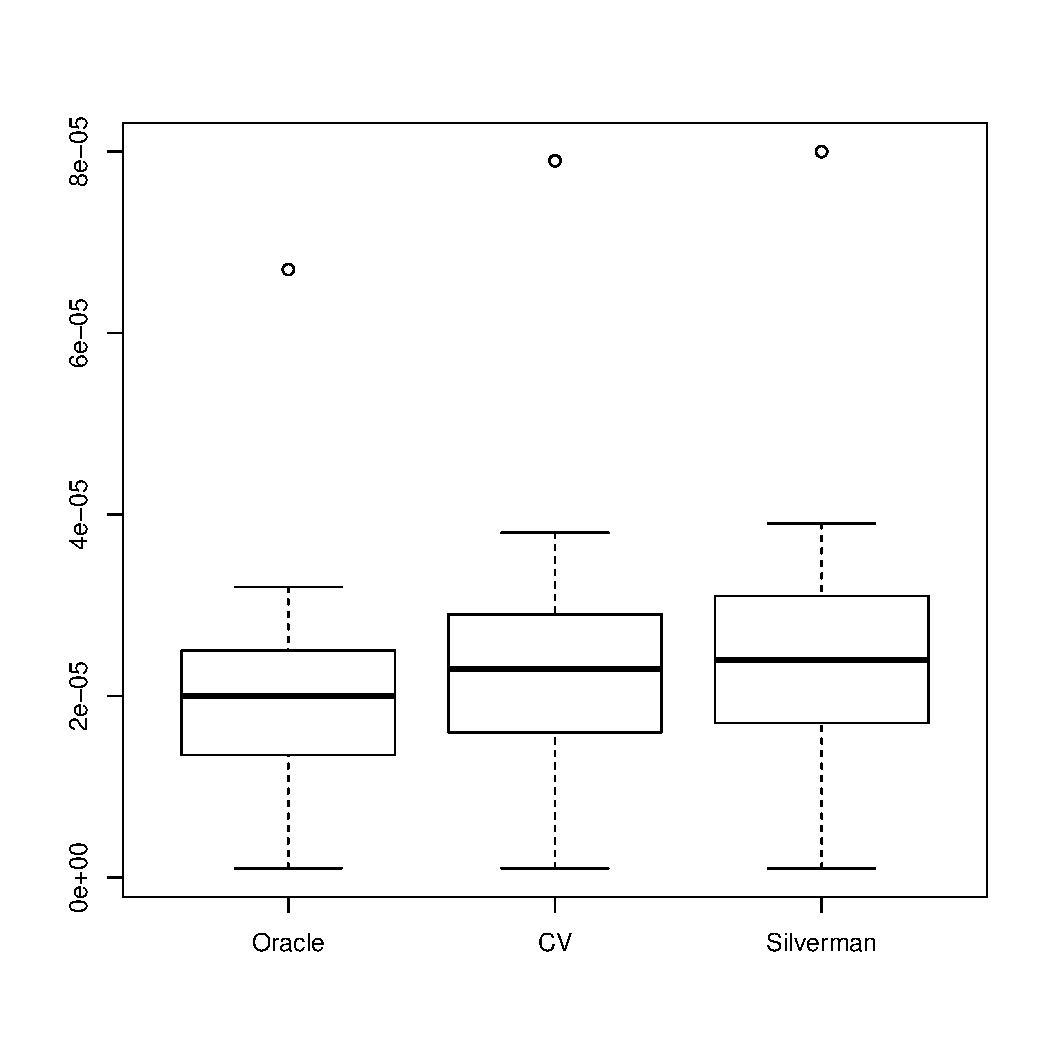
\includegraphics[width=\textwidth]{results/by_overall/normalized-miae-boxplot}
        \subcaption{Uniform populations}
        \label{fig:discussion:overall_nmiae_boxplot:unif}
    \end{subfigure}
    \begin{subfigure}[t]{0.45\textwidth}
        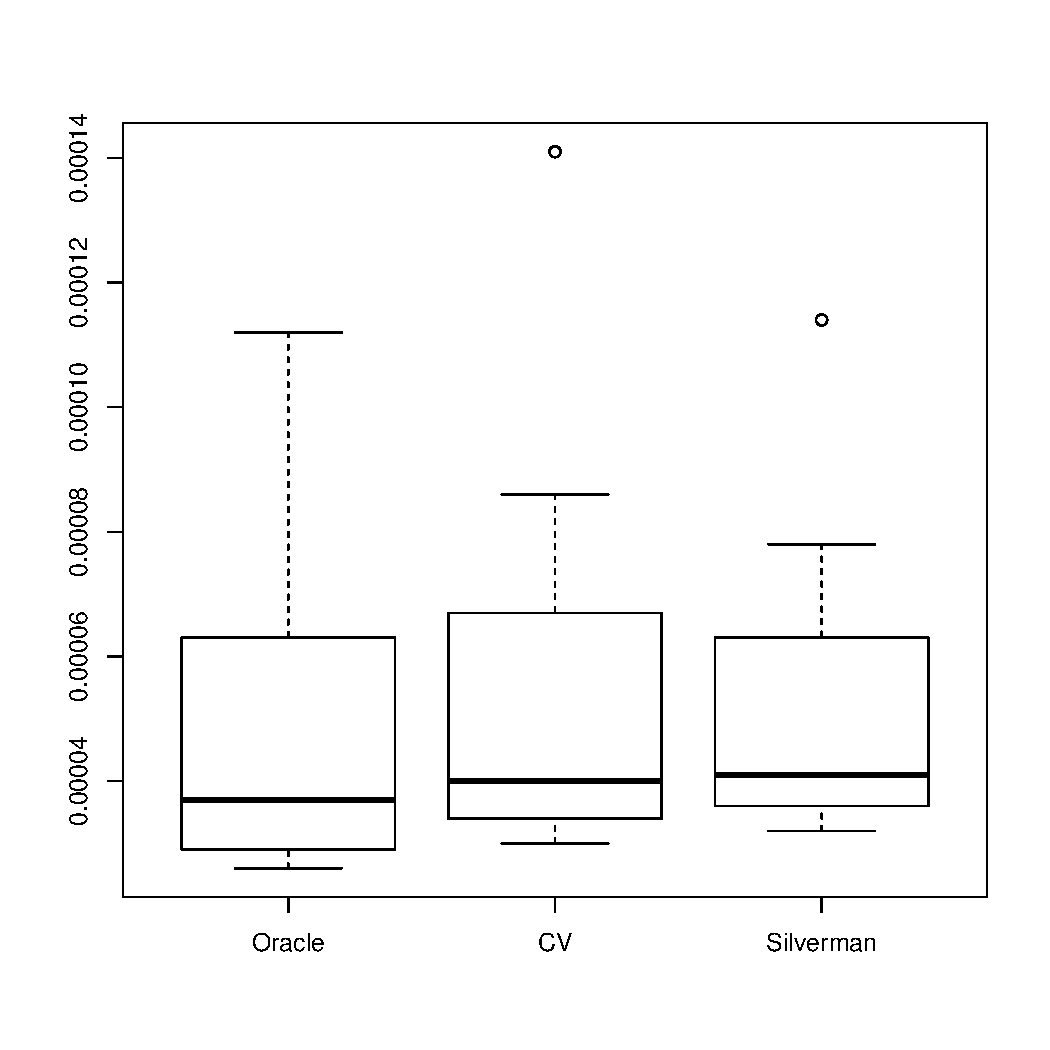
\includegraphics[width=\textwidth]{results/by_overall/normalized-miae-peakpop-boxplot}
        \subcaption{Peaked populations}
        \label{fig:discussion:overall_nmiae_boxplot:peak}
    \end{subfigure}
    \caption{Overall distribution of \glsentryname{nmiae}}
    \label{fig:discussion:overall_nmiae_boxplot}
\end{figure}

\begin{figure}[htbp]
    \centering
    \begin{subfigure}[t]{0.45\textwidth}
        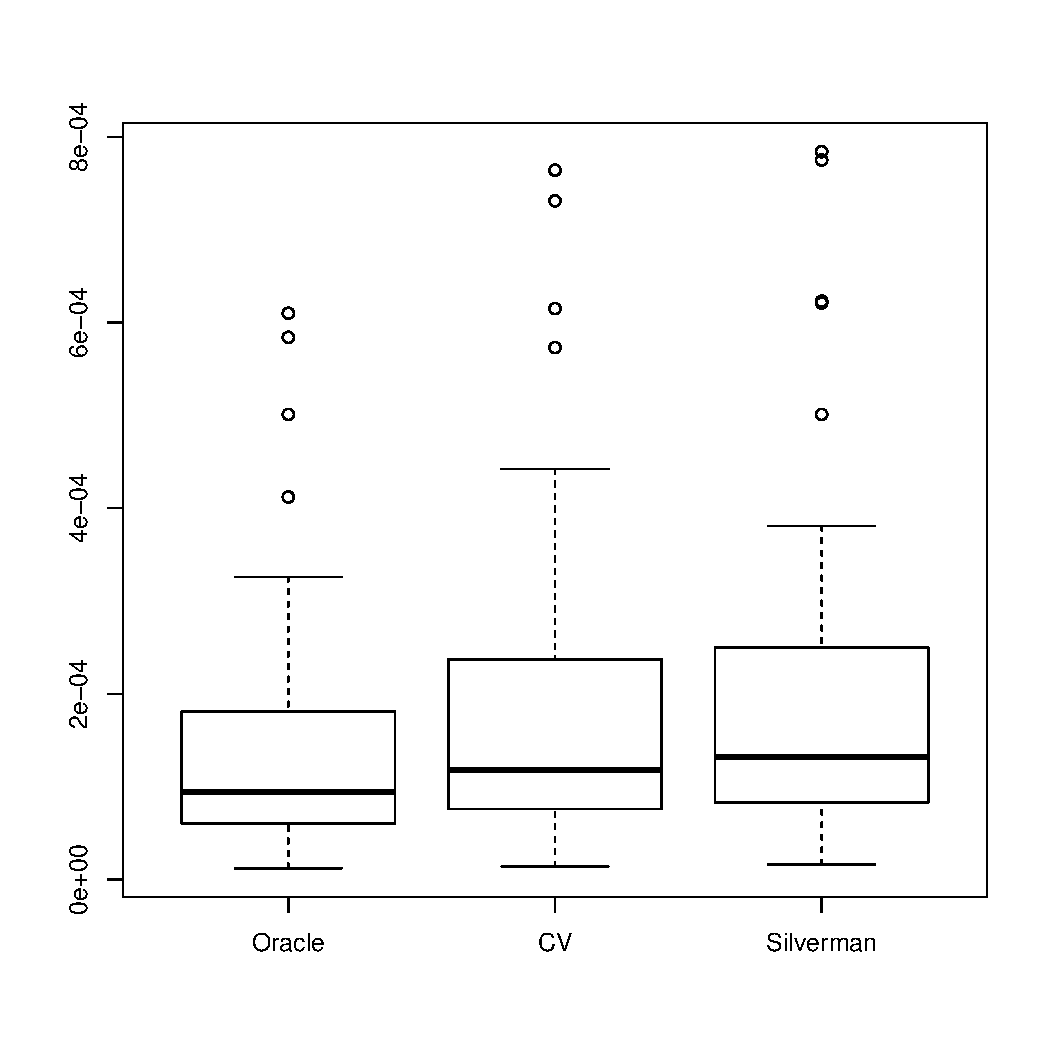
\includegraphics[width=\textwidth]{results/by_overall/normalized-sup-error-boxplot}
        \subcaption{Uniform populations}
        \label{fig:discussion:overall_nsup_boxplot:unif}
    \end{subfigure}
    \begin{subfigure}[t]{0.45\textwidth}
        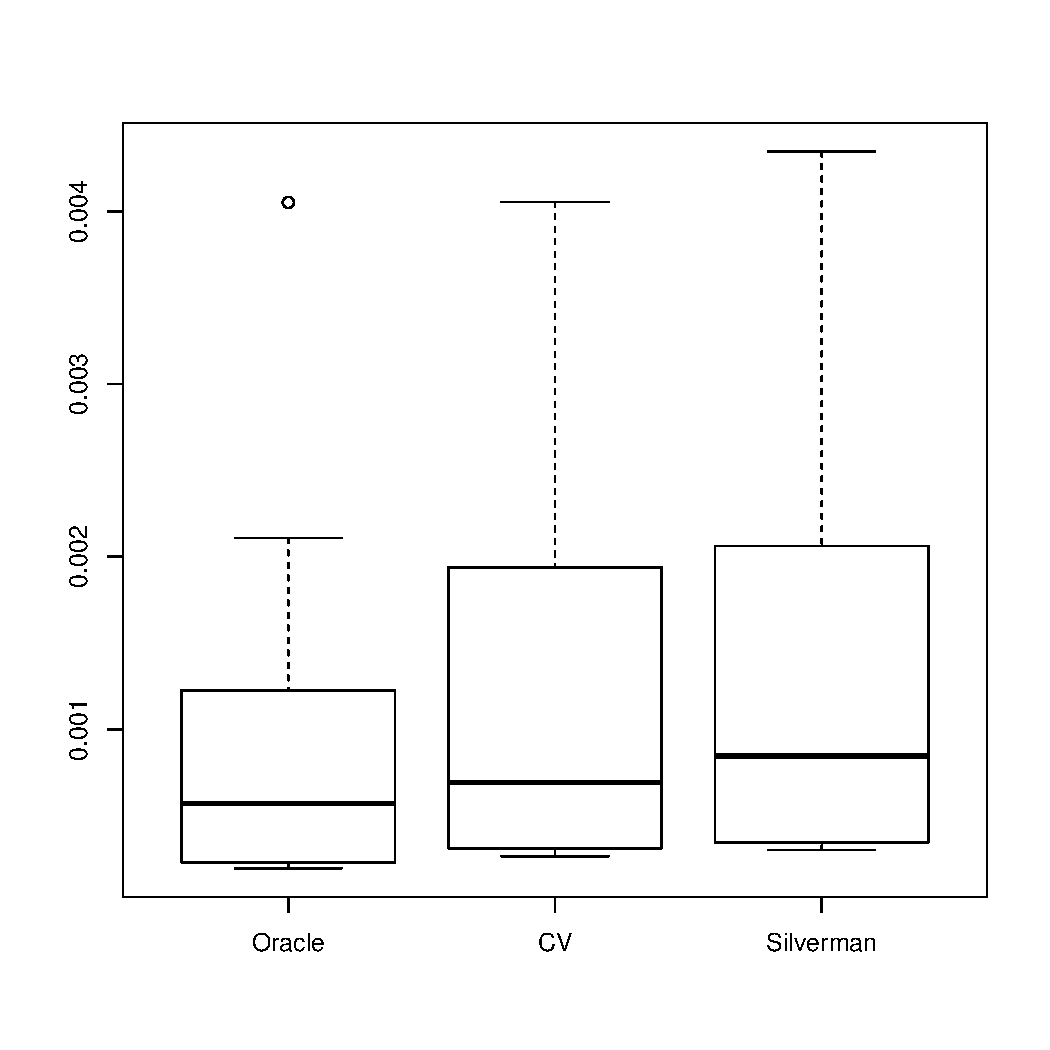
\includegraphics[width=\textwidth]{results/by_overall/normalized-sup-error-peakpop-boxplot}
        \subcaption{Peaked populations}
        \label{fig:discussion:overall_nsup_boxplot:peak}
    \end{subfigure}
    \caption{Overall distribution of \glsentryname{normalized supremum error}}
    \label{fig:discussion:overall_nsup_boxplot}
\end{figure}

Our \gls{supremum error} measure intuitively describes the expected worst case error of the \gls{dkd} estimate.
\Cref{fig:discussion:overall_nsup_boxplot} shows the overall distribution of the \gls{supremum error} over our experiments.
The results for uniform and peaked populations are shown in \Cref{fig:discussion:overall_nsup_boxplot:unif,fig:discussion:overall_nsup_boxplot:peak} respectively.

\begin{figure}[htbp]
    \centering
    \begin{subfigure}[t]{0.45\textwidth}
        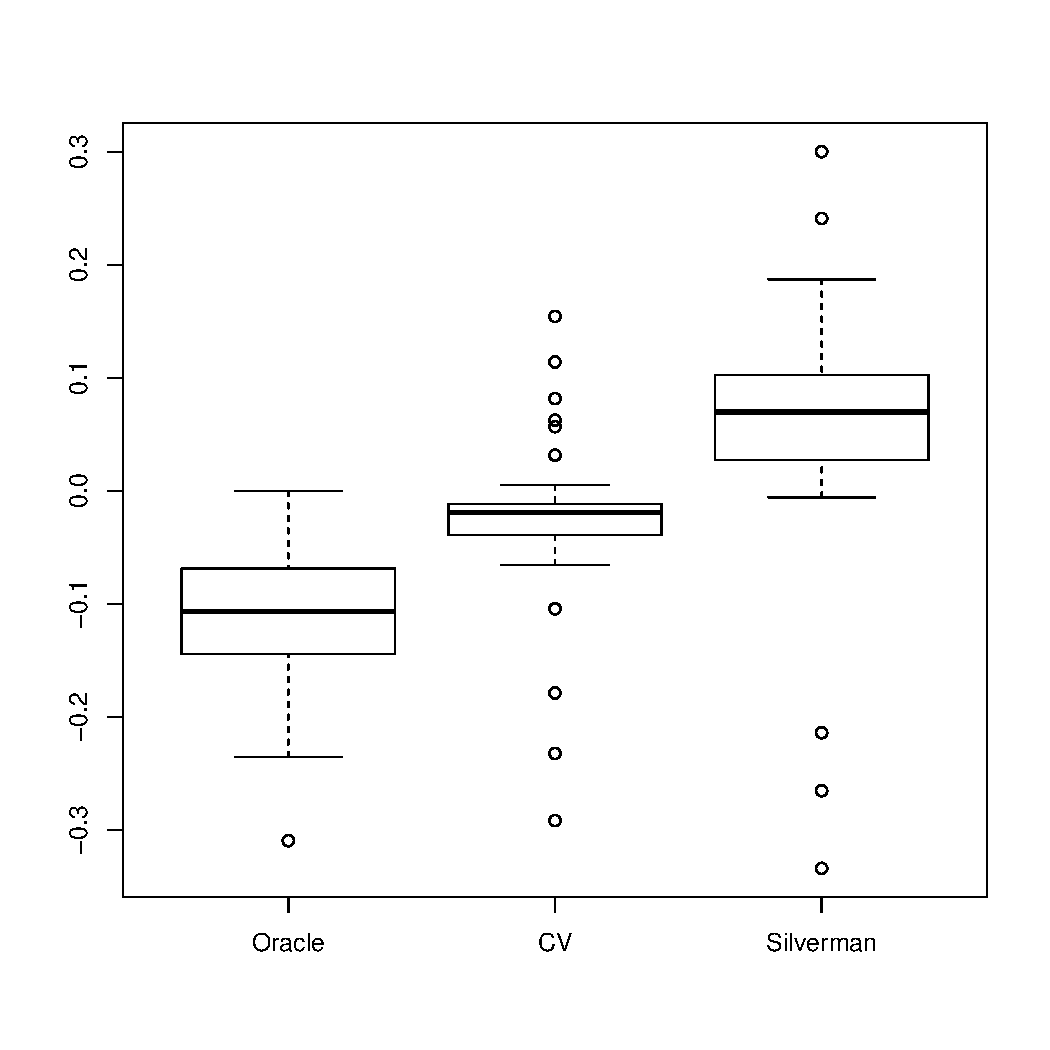
\includegraphics[width=\textwidth]{results/by_overall/relative-peak-bias-boxplot}
        \subcaption{Uniform populations}
        \label{fig:discussion:overall_peakbias_boxplot:unif}
    \end{subfigure}
    \begin{subfigure}[t]{0.45\textwidth}
        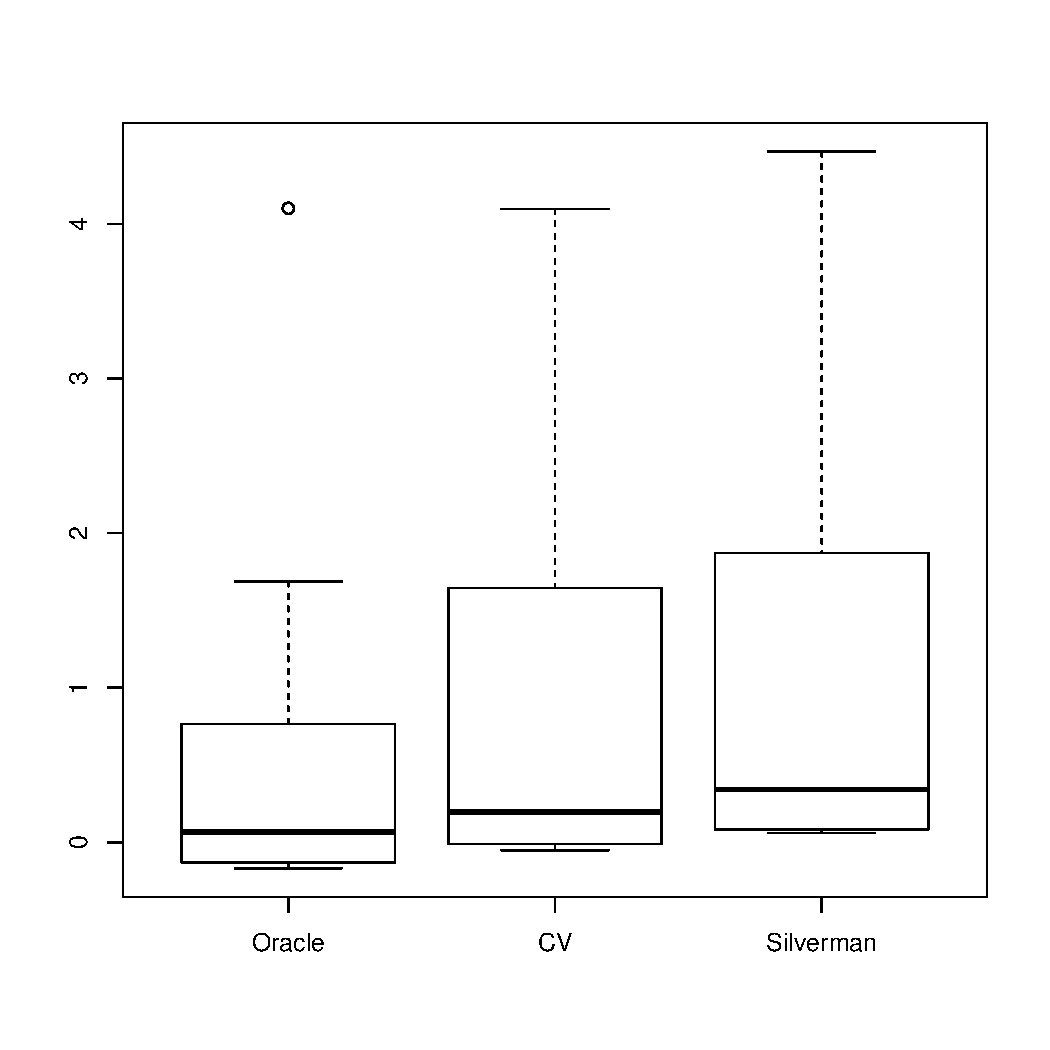
\includegraphics[width=\textwidth]{results/by_overall/relative-peak-bias-peakpop-boxplot}
        \subcaption{Peaked populations}
        \label{fig:discussion:overall_peakbias_boxplot:peak}
    \end{subfigure}
    \caption{Overall distribution of relative \glsentryname{peak bias}}
    \label{fig:discussion:overall_peakbias_boxplot}
\end{figure}

\begin{figure}[htbp]
    \centering
    \begin{subfigure}[t]{0.45\textwidth}
        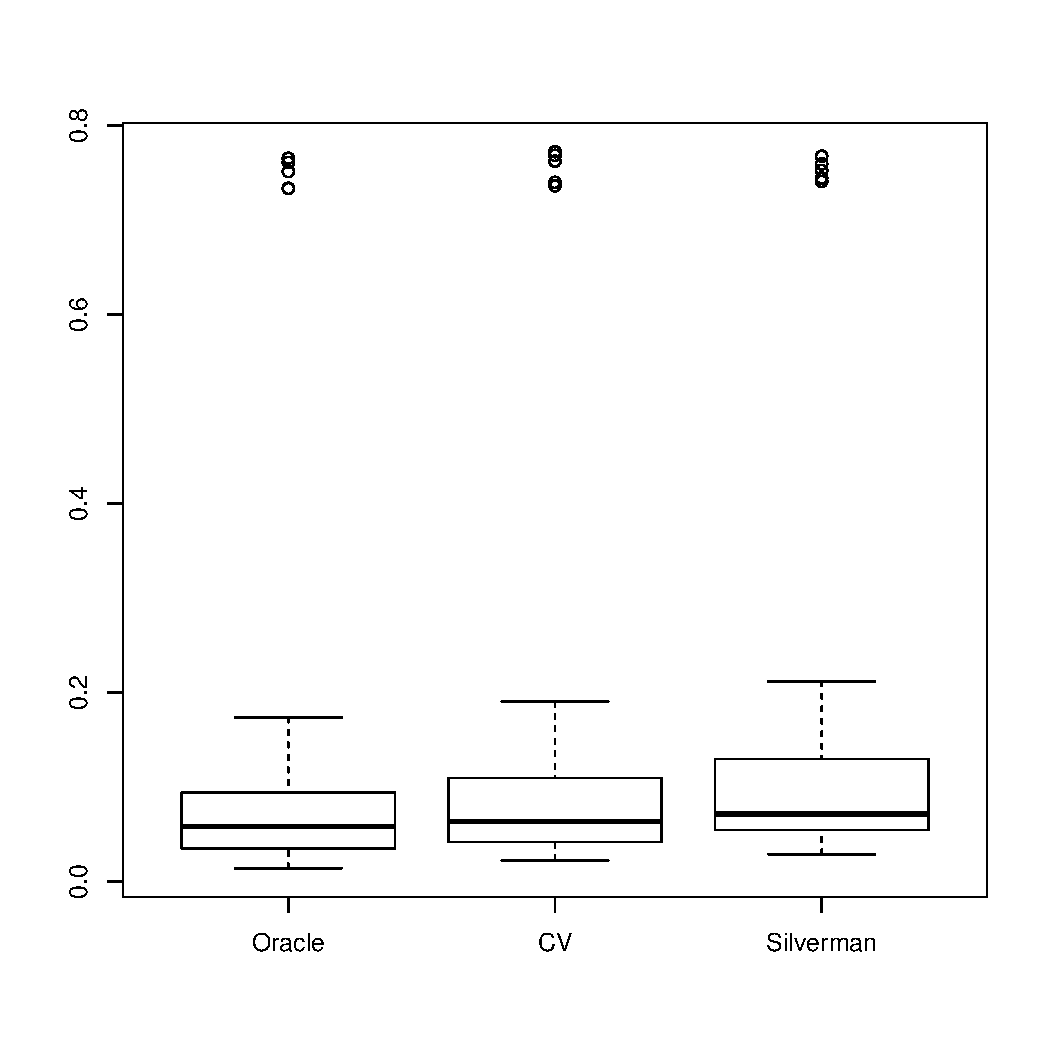
\includegraphics[width=\textwidth]{results/by_overall/relative-peak-drift-boxplot}
        \subcaption{Uniform populations}
        \label{fig:discussion:overall_peakdrift_boxplot:unif}
    \end{subfigure}
    \begin{subfigure}[t]{0.45\textwidth}
        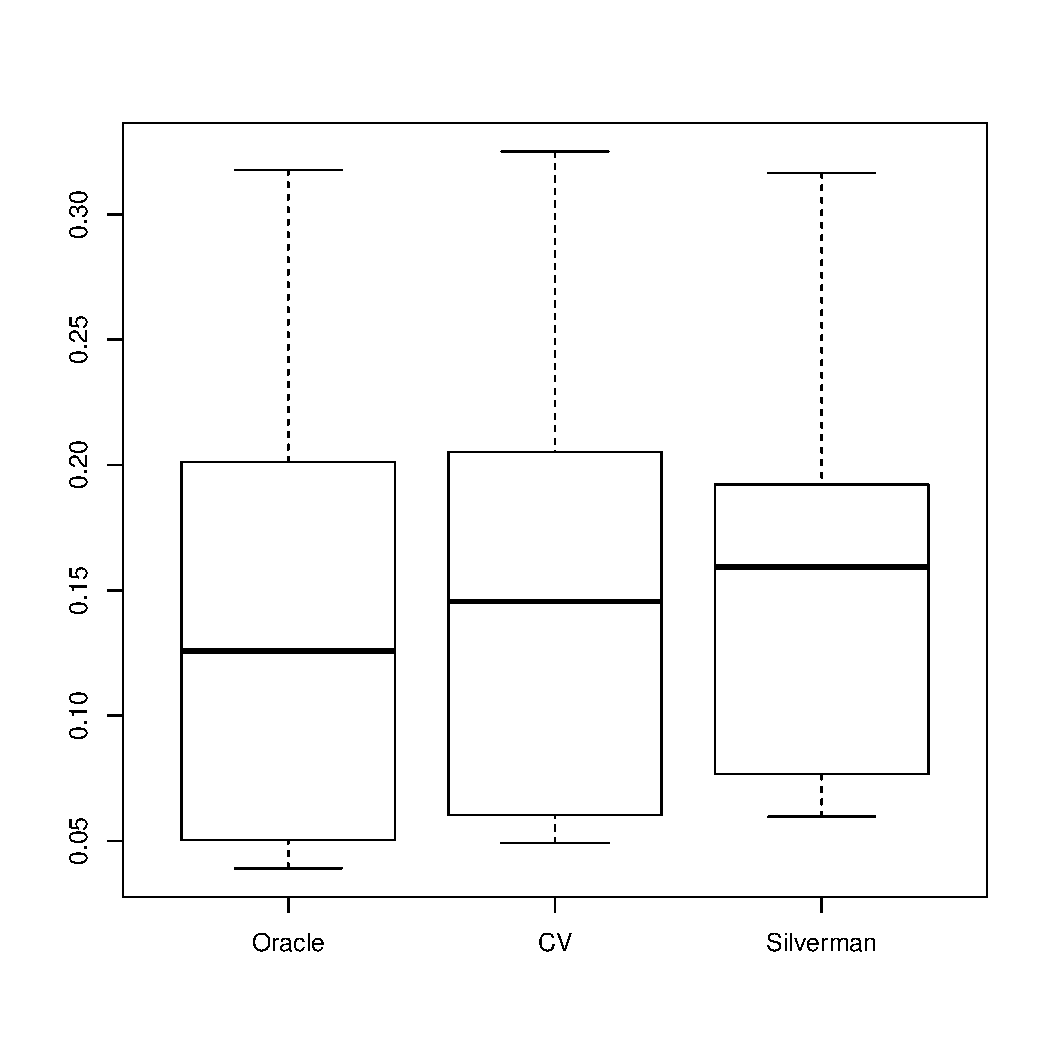
\includegraphics[width=\textwidth]{results/by_overall/relative-peak-drift-peakpop-boxplot}
        \subcaption{Peaked populations}
        \label{fig:discussion:overall_peakdrift_boxplot:peak}
    \end{subfigure}
    \caption{Overall distribution of relative \glsentryname{peak drift}}
    \label{fig:discussion:overall_peakdrift_boxplot}
\end{figure}

The distributions we observed for \gls{peak bias} and \gls{peak drift} are shown in \Cref{fig:discussion:overall_peakbias_boxplot,fig:discussion:overall_peakdrift_boxplot}.
First, we note that the \gls{peak bias} is always negative when computing the \gls{dkd} with the \gls{oracle} bandwidth,
for uniformly distributed populations.
This is in line with what we would expect,
as, in general, we expect smoothing techniques to underestimate high values and overestimate low values.
For the \gls{cv} selected bandwidths, this is the case for the mean and for the majority of cases.
However, we see that for the \gls{silverman} bandwidths,
most of the values for \gls{peak bias} are positive,
indicating a tendency to undersmooth.

For the peaked population experiments, all of the bandwidth selection techniques including the \gls{oracle} resulted in positive \gls{peak bias}.
This needs further investigation.

\begin{figure}[htbp]
    \centering
    \begin{subfigure}[t]{0.45\textwidth}
        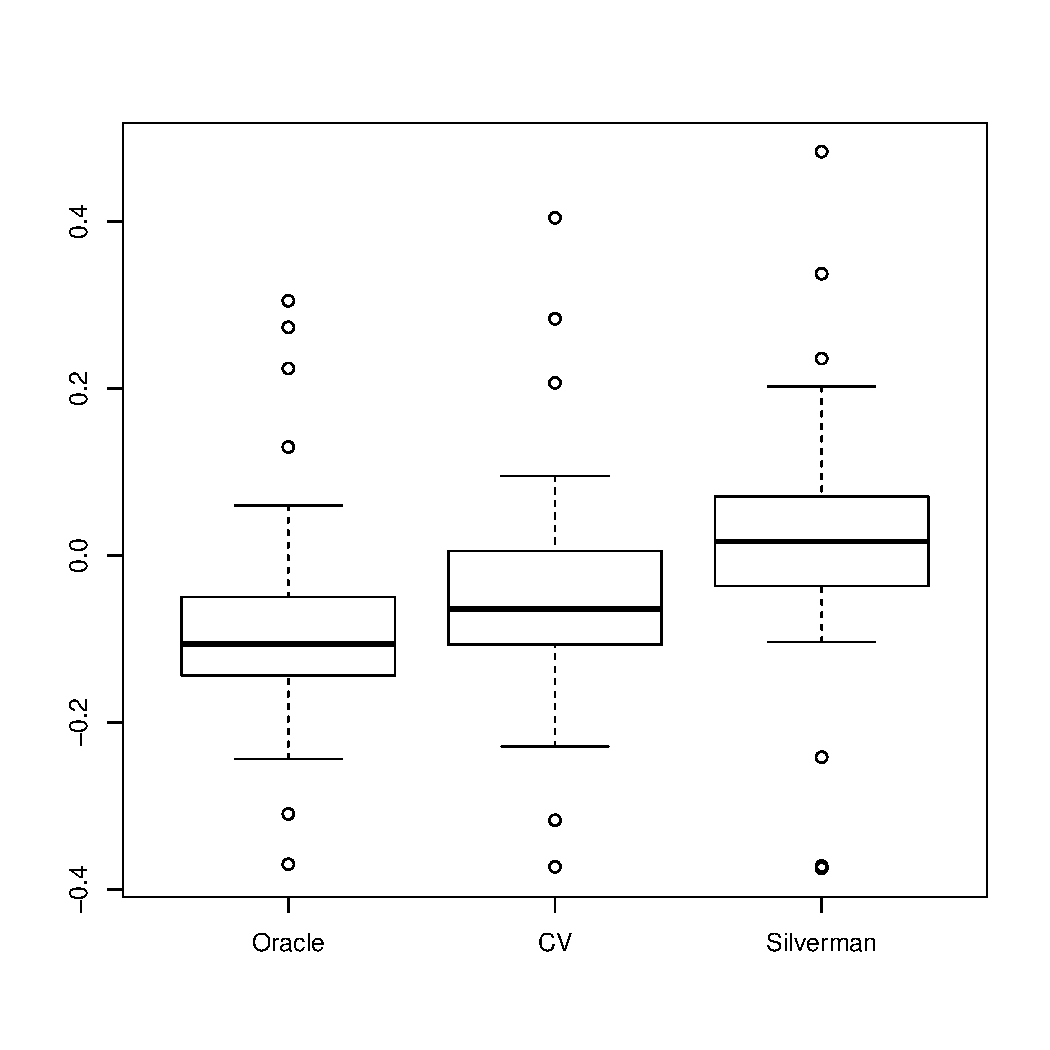
\includegraphics[width=\textwidth]{results/by_overall/relative-centroid-bias-boxplot}
        \subcaption{Uniform populations}
        \label{fig:discussion:overall_centroidbias_boxplot:unif}
    \end{subfigure}
    \begin{subfigure}[t]{0.45\textwidth}
        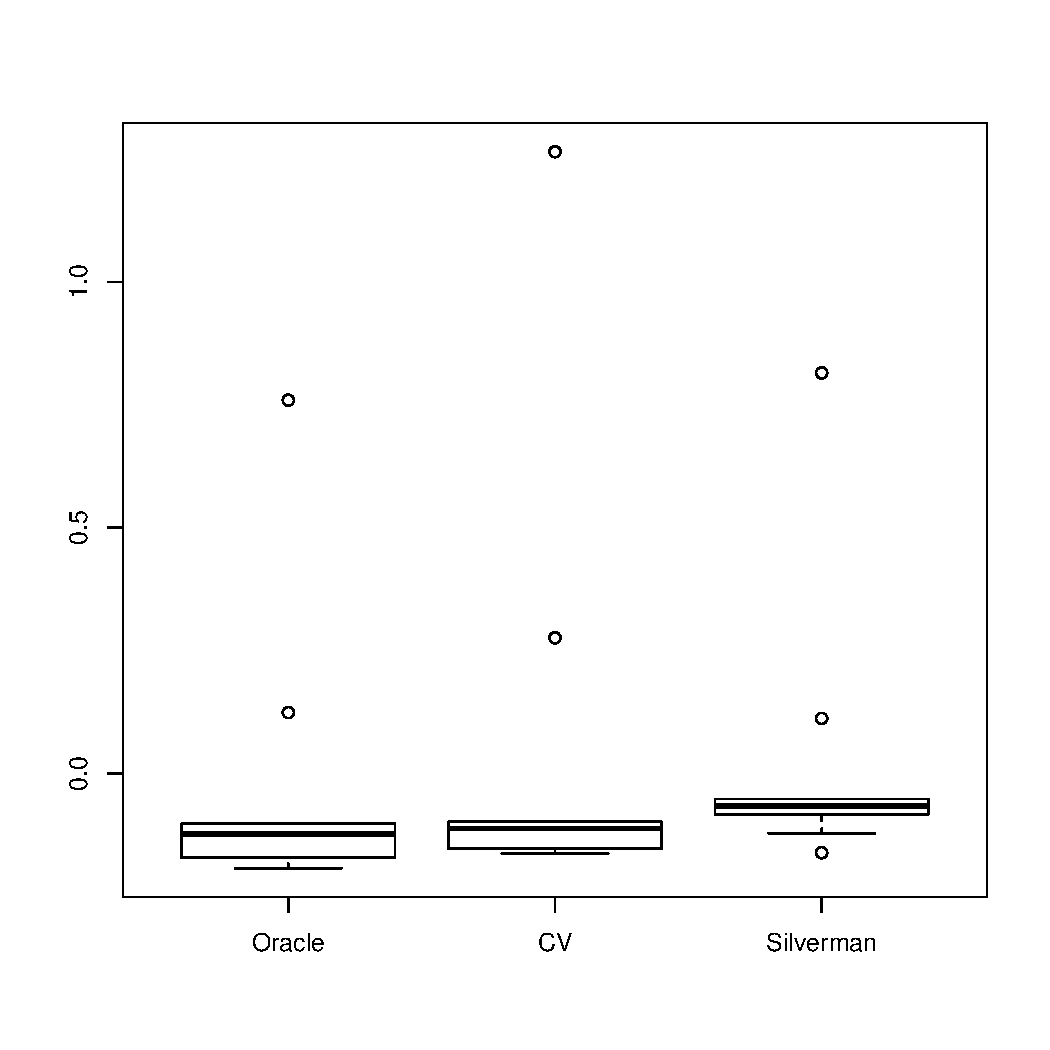
\includegraphics[width=\textwidth]{results/by_overall/relative-centroid-bias-peakpop-boxplot}
        \subcaption{Peaked populations}
        \label{fig:discussion:overall_centroidbias_boxplot:peak}
    \end{subfigure}
    \caption{Overall distribution of relative \glsentryname{centroid bias}}
    \label{fig:discussion:overall_centroidbias_boxplot}
\end{figure}

\begin{figure}[htbp]
    \centering
    \begin{subfigure}[t]{0.45\textwidth}
        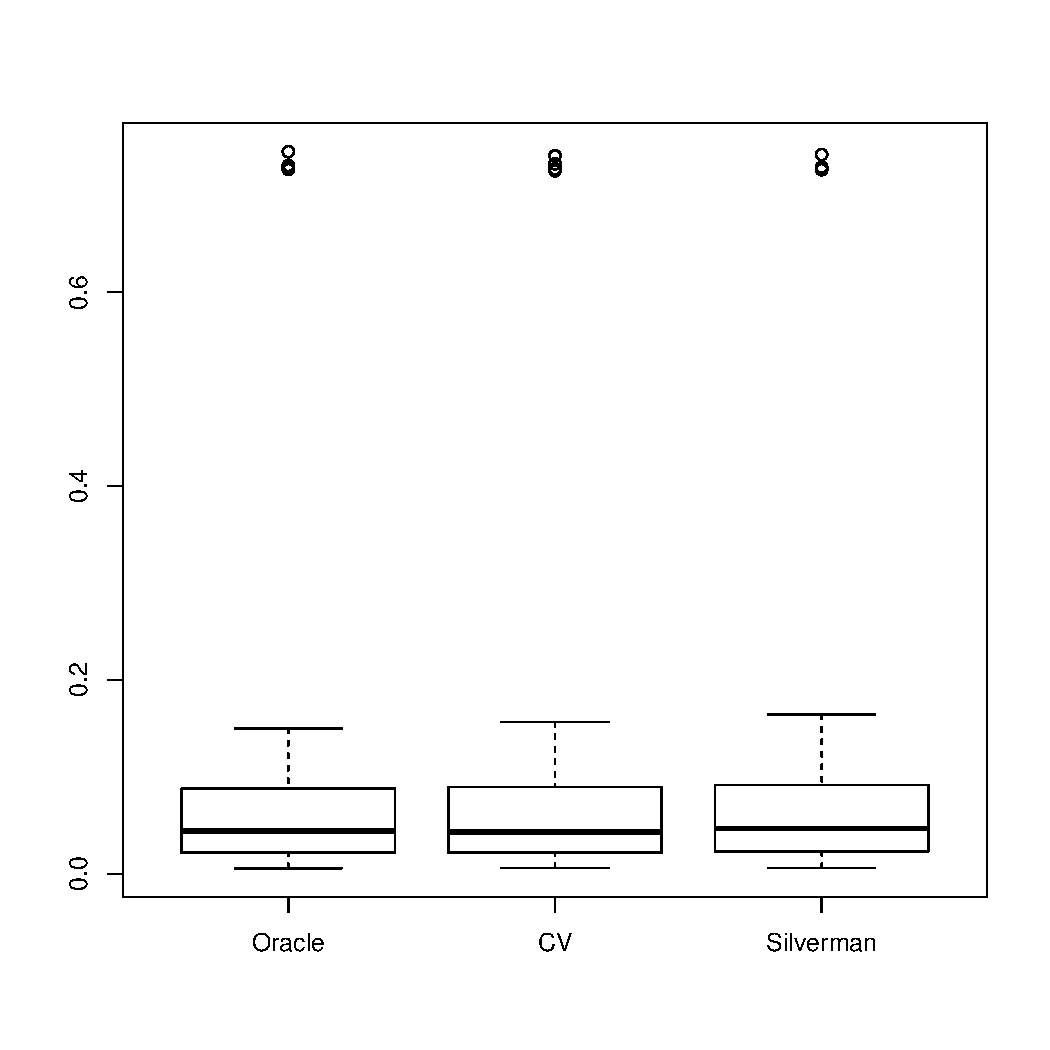
\includegraphics[width=\textwidth]{results/by_overall/relative-centroid-drift-boxplot}
        \subcaption{Uniform populations}
        \label{fig:discussion:overall_centroiddrift_boxplot:unif}
    \end{subfigure}
    \begin{subfigure}[t]{0.45\textwidth}
        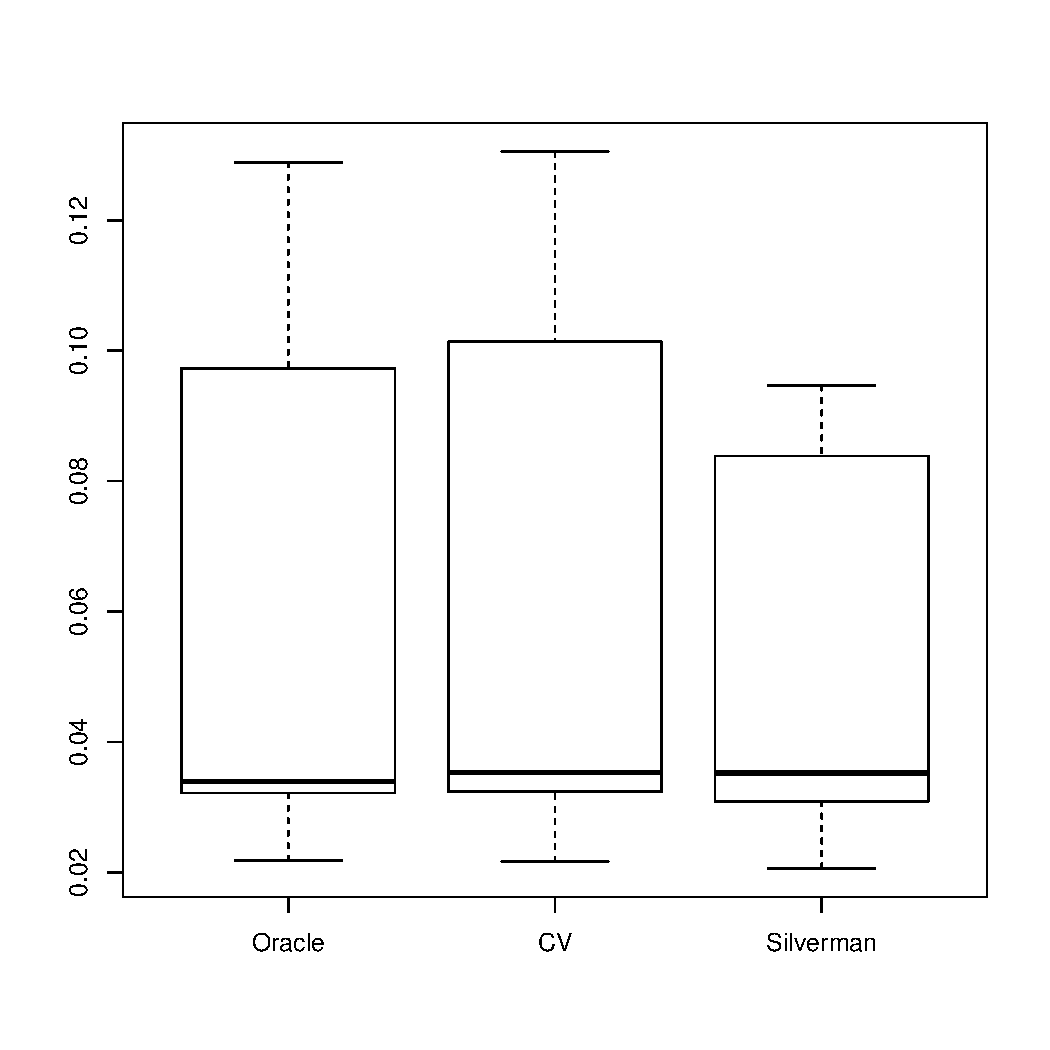
\includegraphics[width=\textwidth]{results/by_overall/relative-centroid-drift-peakpop-boxplot}
        \subcaption{Peaked populations}
        \label{fig:discussion:overall_centroiddrift_boxplot:peak}
    \end{subfigure}
    \caption{Overall distribution of relative \glsentryname{centroid drift}}
    \label{fig:discussion:overall_centroiddrift_boxplot}
\end{figure}

The \gls{centroid bias} performed much better than the \gls{peak bias} for measuring the highest risk.
For the \gls{oracle} selected bandwidths, the distribution was similar to the \gls{peak bias} for uniform populations but much better for populations with peaked distributions.
However, for both \gls{silverman} and \gls{cv} bandwidths, the \gls{centroid bias} was consistently lower in both groups.
The \gls{centroid drift} was lower for all bandwidth selection methods for both groups of experiments.
These results indicate that the centroid method of determining the peak may be a better choice for estimating both the magnitude and location of the risk source.
This is indicated by the better performance of both the \gls{centroid bias} and \gls{centroid drift} accuracy measures over the \gls{peak bias} and \gls{peak drift} respectively.

\section{Gradient descent for cross-validation}
\label{sec:discussion:gradient_descent}

We attempted to speed up the cross-validation bandwidth selection by using gradient descent.
We found the gradient descent algorithm often resulted in severe oversmoothing,
as the cross-validation error would decrease slowly as the bandwidth increased.
This required a lot of manual tuning of the learning rate parameter, and so required re-running the experiment several times.
We added \textit{momentum} to our gradient descent implementation but it did not help in every case, and so we changed our strategy to the one described in \Cref{ch:method}.

\section{Accuracy using Silverman}

In \Cref{tab:mean_error_rates:p0.7_100_1.0_1h} we see that the accuracy measure \gls{mise} using the \gls{silverman} rule of thumb is even better than was obtained using the \gls{oracle}.
We tried to run with an additional experiment with 499 monte carlo simulations, and found that in this case the \gls{silverman} rule did not outperform the \gls{oracle}.

\section{Summary}

We used monte carlo simulations to empirically estimate the accuracy of the \acrlong{dkd} estimate of simulated disease risk intensity functions.
For this, we used several accuracy measures that measure the overall accuracy as well as the accuracy of the peak.
We also used two bandwidth selection methods to choose the bandwidth of the \gls{dkd}.
We did this while varying several factors.
In \Cref{sec:results:number_of_incidents} increasing the \gls{factor} resulted in decreased selected bandwidths
and increase relative accuracy, although absolute accuracy decreased.
Increasing the incidence \gls{spread} also resulted in increased relative accuracy.
Increasing the population size also resulted in increased accuracy,
while changing the population \gls{spread} resulted in unpredictable accuracy measures.
These results are interesting,
and there are are many opportunities for further work.


